\section{HXRM firmware}

Based on the results of the research and simulations, the best timing
and shaping algorithms were implemented in hardware.
The ADQ14 uses Verilog and Vivado 2015.2, so these tools
were chosen for the implementation of the HXRM.
The developed system performs pulse detection,
measures the peak height, stores the resultant spectrum
and periodically transfers the results to the host PC.

\subsection{System overview}

As described in \autoref{ssec:adq_devkit} the ADQ14 DevKit
grants a semi-open FPGA design with two modules that can be
freely modified by the end user. The board manufacturer
designed User Logic 1 with intent for it to house timing filters
and User Logic 2 to contain more specialized processing logic.
Initially, these ideas were followed with a Boxcar filter being
implemented in User Logic 1 and a Pulse Height Analyzer being placed 
in User Logic 2.


With the default firmware, ADQ14 generates fixed-length records
on trigger events. For example, with the window length set to a 1000
samples, upon the detection of a pulse, 1000 samples would always be
transferred to the PC, irregardless of pile ups and other disturbances.
For this reason the timing logic originally placed in User Logic 1 was moved
to User Logic 2, so that it could be better integrated with the rest 
of the pulse analysis systems. The UL2 module allows for full control 
over record lengths, so sampling windows, in which pile ups were detected,
could now be rejected, split into two or combined.
\autoref{fig:firmware_overview} gives an overview of the system designed
in User Logic 2.

\begin{figure}[H]
  \centering
  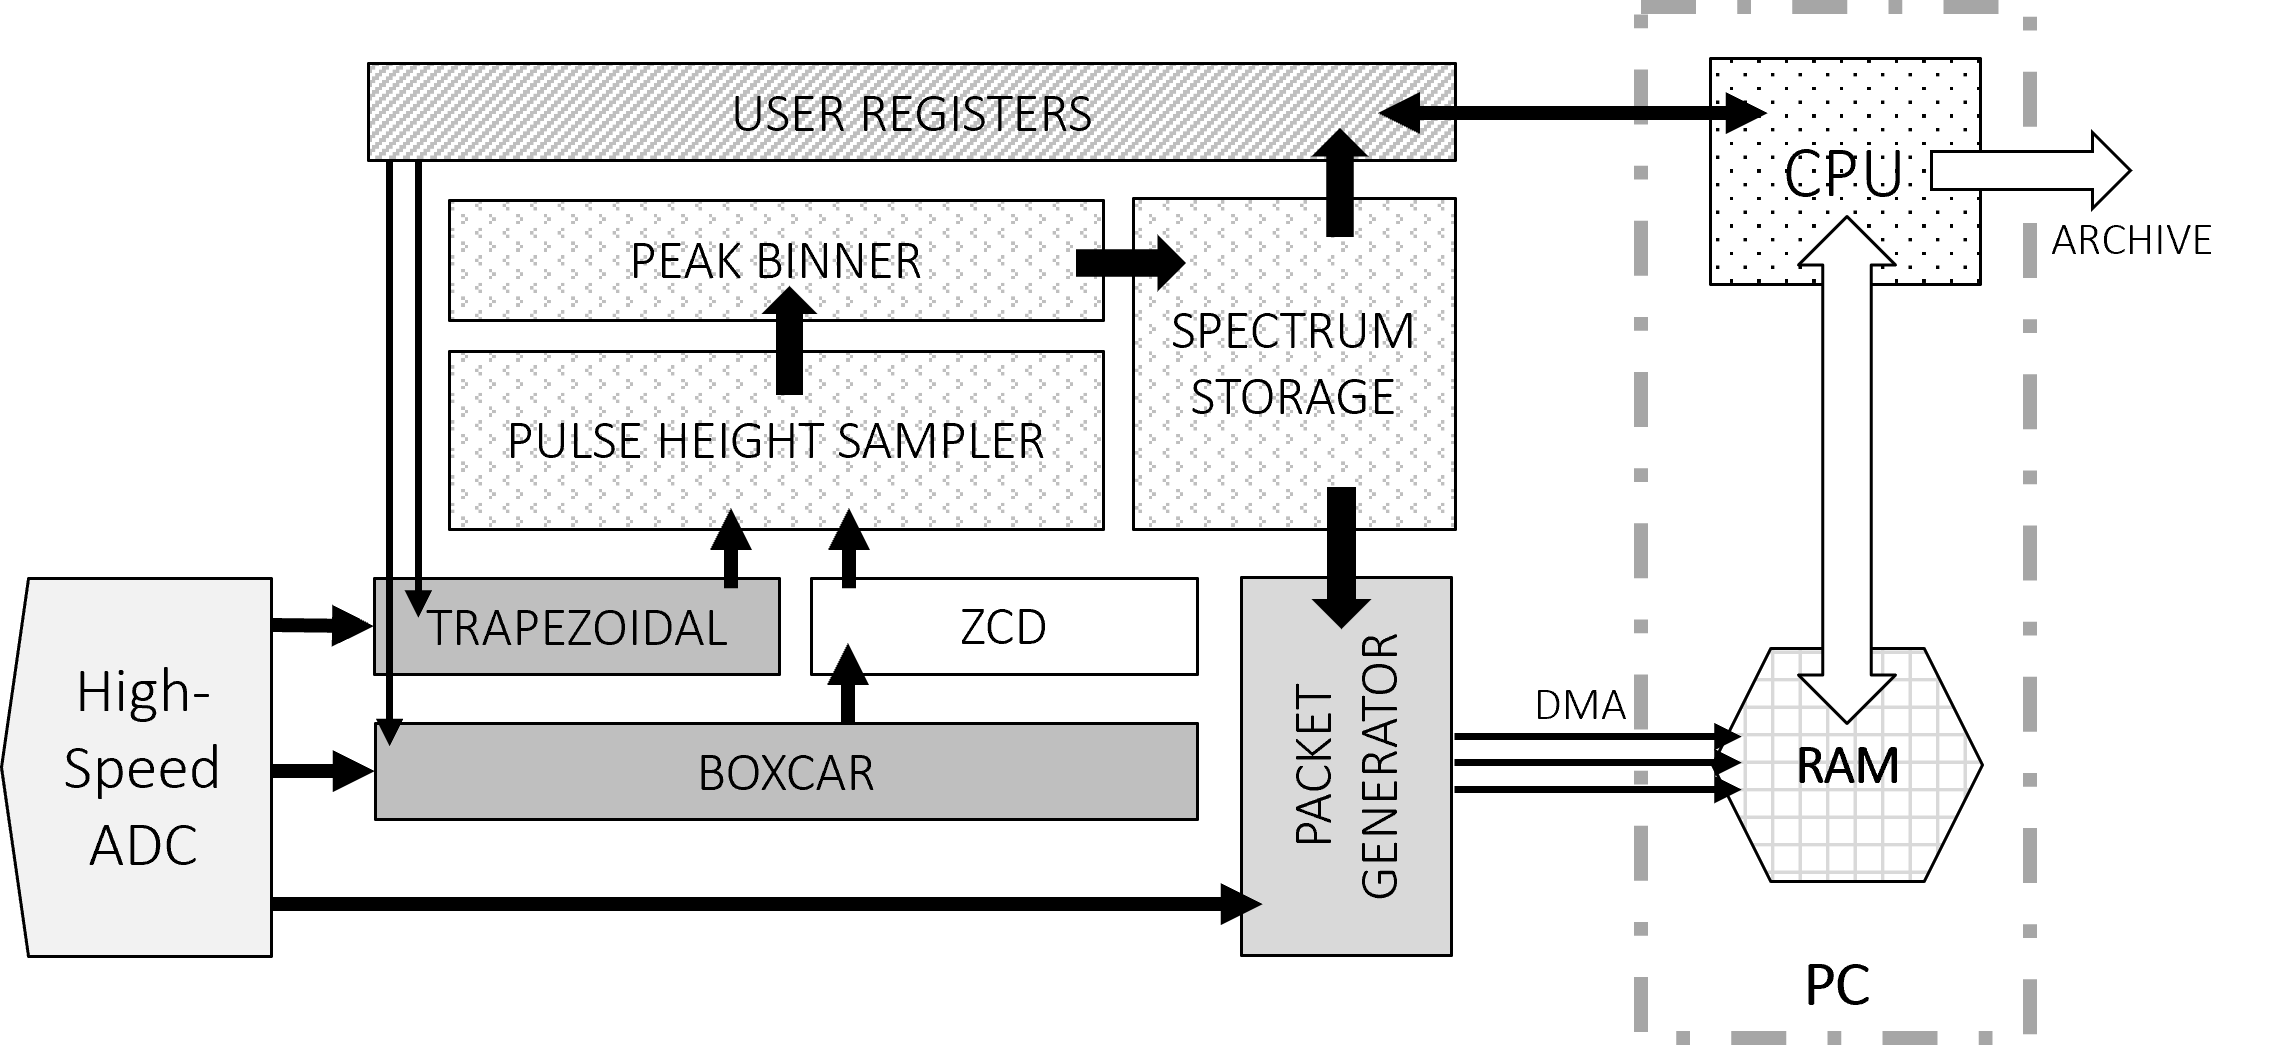
\includegraphics[width=\linewidth]{media/fpga_system_trap.png}
  \caption{Firmware overview in User Logic 2}
  \label{fig:firmware_overview} 
\end{figure}
\subsection{System control}

The system is configured and controlled with the use of so called 
user registers. $2^{19}$ individually addressable 32-bit words
are available for reading and writing to from the PC. The first
four words are reserved for internal use by the ADQ library. 
In the custom design, the next four have been 
dedicated for configuration and control as listed in \autoref{tab:ureg_control}.
The $2^{14}$ block of addresses starting from position 9, can
be used to read the currently held spectrum.

\begin{table}[H]
\caption{User register addresses}
\centering
  \begin{tabular}{l | l | l}
  {\bfseries Address} & {\bfseries Bits} & {\bfseries Description}\\
  \hline
  0-3  & *      & \textit {ADQ14 Reserved}\\ \hline
  4    & 0-31       & \textit {ZCD threshold level}\\ \hline
  5    & 0-31       & \textit {Analog DC bias}\\ \hline
  6    & 0       & \textit {PHA enable}\\ \hline
  6    & 1       & \textit {PHA reset}\\ \hline
  6    & 2       & \textit {ZCD trigger enable}\\ \hline
  6    & 3       & \textit {Windowed spectrum enable}\\ \hline
  6    & 4-15  & \textit {Reserved for future use}\\ \hline
  6    & 16-31   & \textit {Record length}\\ \hline
  7    & 0-15   & \textit {Spectrum window length}\\ \hline
  7    & 28-31   & \textit {Spectrum bin count reduction}\\ \hline
  8    & *  & \textit {Reserved for future use}\\ \hline
  9-16392    & *   & \textit {Long window spectrum counts}\\ 
  \end{tabular}
  \label{tab:ureg_control}
\end{table}

\subsection{Pulse detection}
The pulse detection module relies on the use of a configurable boxcar filter
that then passes through a zero crossing detector. Depending on the
length of the boxcar window the result of the ZCD is delayed by an appropriate
amount so that it points to a point at which the trapezoidal filter's 
rising edge starts. To prevent false triggers the ZCD operates in two modes.
First it awaits a user specified threshold value to be crossed. Only after
that event occurs, does it start looking for a zero crossing.
After a zero crossing the system returns back to the threshold awaiting state.
\autoref{fig:zcd_algorithm} illustrates this algorithm. 
The threshold value is set through user registers and does not require
the FPGA to be reprogammed to be modified.

\begin{figure}[H]
  \centering
  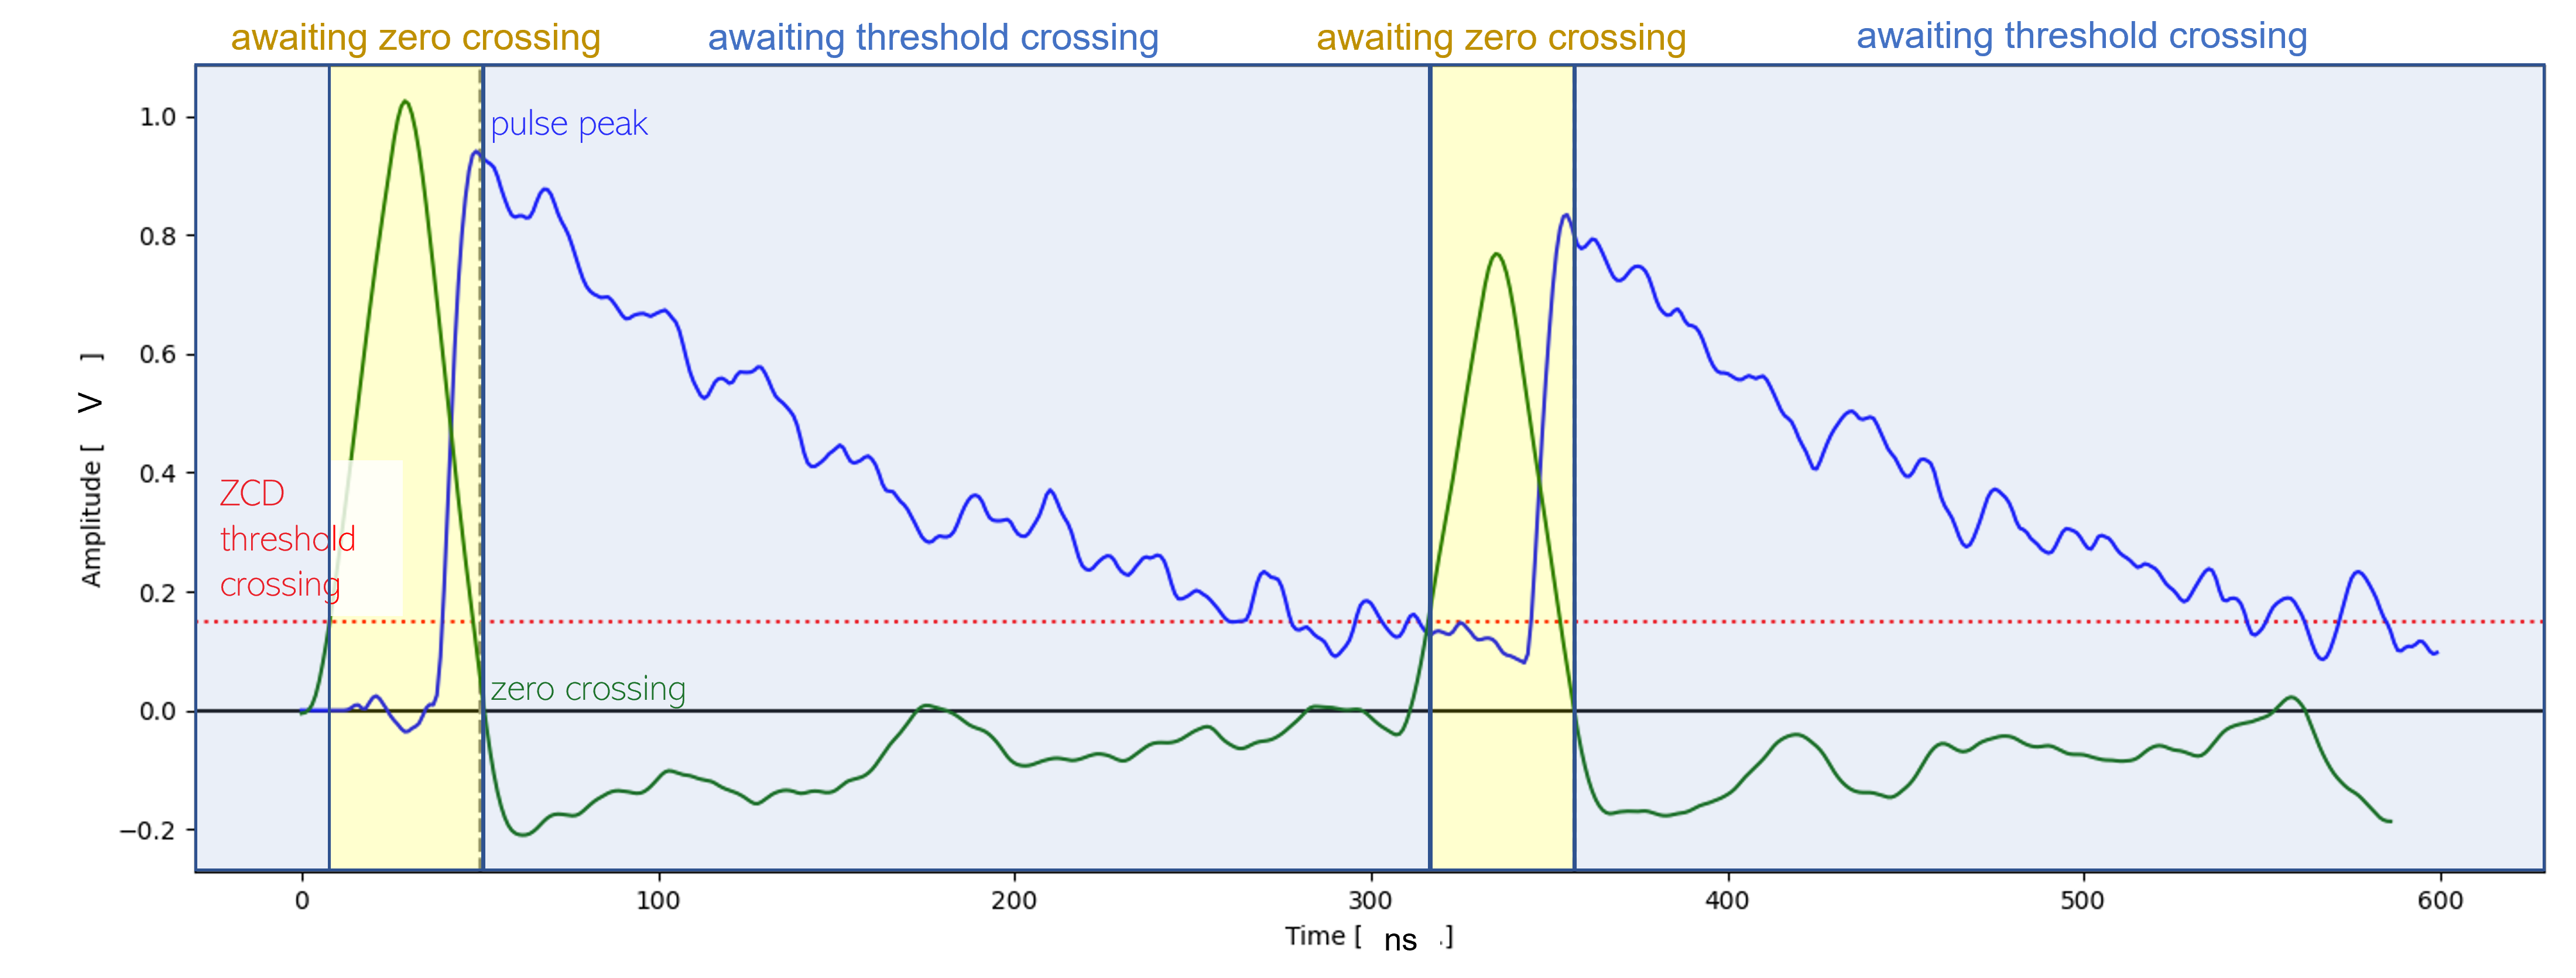
\includegraphics[width=\linewidth]{media/zcd_algorithm.png}
  \caption{Zero Crossing Detection algorithm employed in firmware for pulse detection and timing}
  \label{fig:zcd_algorithm} 
\end{figure}


The implementation of a boxcar filter in firmware required a few considerations
due to the parallel sampling described in \autoref{sssec:parallel_sampling}.
The general formula for a boxcar filter can be described as follows:
$$y(n) = \frac{1}{W} \sum^n_{i=n-W+1}x(i) - \sum^{n-W}_{i=n-2W+1}x(i)$$
$W$ stands for the boxcar window length and $x(n)$ is the input signal.
The mathematical formula requires the use of two moving average filters.
The pseudocode below describes the Register Transfer Level behaviour 
used to implement an optimized Moving Average filter in firmware.

\begin{lstlisting}
for parsamp in [3...0]:
  ma_0[parsamp] <= x[parsamp] - x[parsamp+W];
ma_1[3] <= ma_0[3];
ma_1[2] <= ma_0[3] + ma_0[2];
ma_1[1] <= ma_0[1];
ma_1[0] <= ma_0[1] + ma_0[0];
ma_2[3] <= ma_1[3];
ma_2[2] <= ma_1[2];
ma_2[1] <= ma_1[2] + ma_1[1];
ma_2[0] <= ma_1[2] + ma_1[0];
for parsamp in [3...0]:
	ma_3[parsamp] <= ma_3[0] + ma_2[parsamp];
	divided[parsamp] <= ma_3[parsamp] / W;
	y[parsamp] <= divided[parsamp] - divided[parsamp+W];
\end{lstlisting}


Four parallel samples are available on each clock cycle. To obtain
an average they all must be added together. This requires the design
to use pipelining. Attempting to add up 4 16-bit integers within a single clock cycle
would violate the timing constraints specified by the FPGA. In other words,
the synthesis tool can not route such a path in the device
that this addition would reliably execute at the 250 MHz clock frequency.


As the first step, a moving average is calculated for each parallel sample 
as if the given sample was the only sample generated on each clock cycle. 
One sample now outside the MA window is subtracted and a new sample
is added to the current rolling sum. In the next pipeline steps 
the four parallel samples are added together. The proposed algorithm
relies solely on two operand addition and requires one less clock cycle
when compared to a simple cascading addition. 


As the penultimate step a division over the window length is made.
Integer division is a very costly operation in terms of hardware usage.
It can, however, be avoided if the allowable window lengths are limited to 
natural powers of 2. In such case a division is equivalent to a  
right bitshift by a number equal to the power exponent.
A 16-bit integer divider requires around 20 clock cycles to produce a result.
A bitshift can be very efficiently performed within a single clock cycle.


Finally, to obtain the boxcar, the divided values are delayed by the
window length and subtracted. \autoref{fig:accumulator} shows
the optimized accumulator being realized with DSP blocks.

\begin{figure}[H]
  \centering
  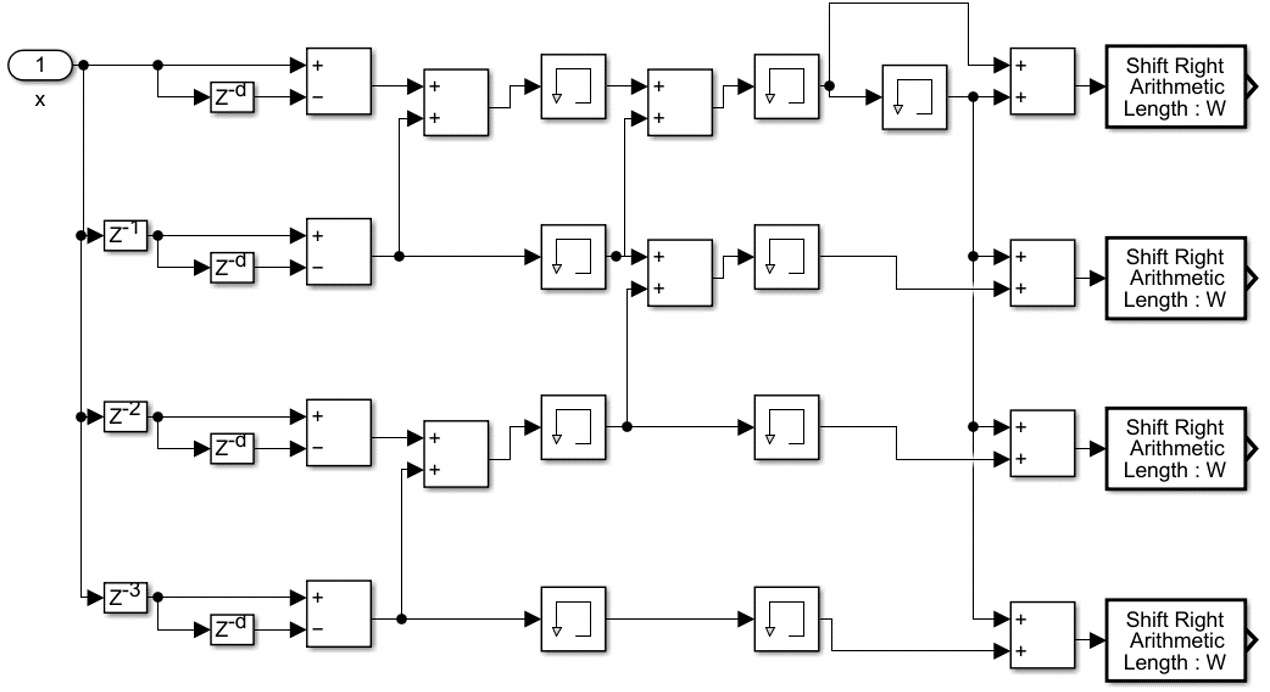
\includegraphics[width=\linewidth]{media/accumulator.png}
  \caption{Timing optimized accumulator}
  \label{fig:accumulator} 
\end{figure}

\subsection{Pulse height analysis}

The timing generated by the ZCD is resynchronized to a trapezoidal filter, 
to indicate the start of the trapezoid. After a delay equal to the 
trapezoid edge the peak sampling module activates. The module
accumulates every sample from the trapezoid flattop and 
divides the end result by the number of samples.
The result grants an average flattop height that corresponds
to the pulse peak height. The averaging action reduces overall noise
and increases the measurement's precision.
\autoref{fig:pha_algorithm} visualizes the PHA algorithm.

\begin{figure}[H]
  \centering
  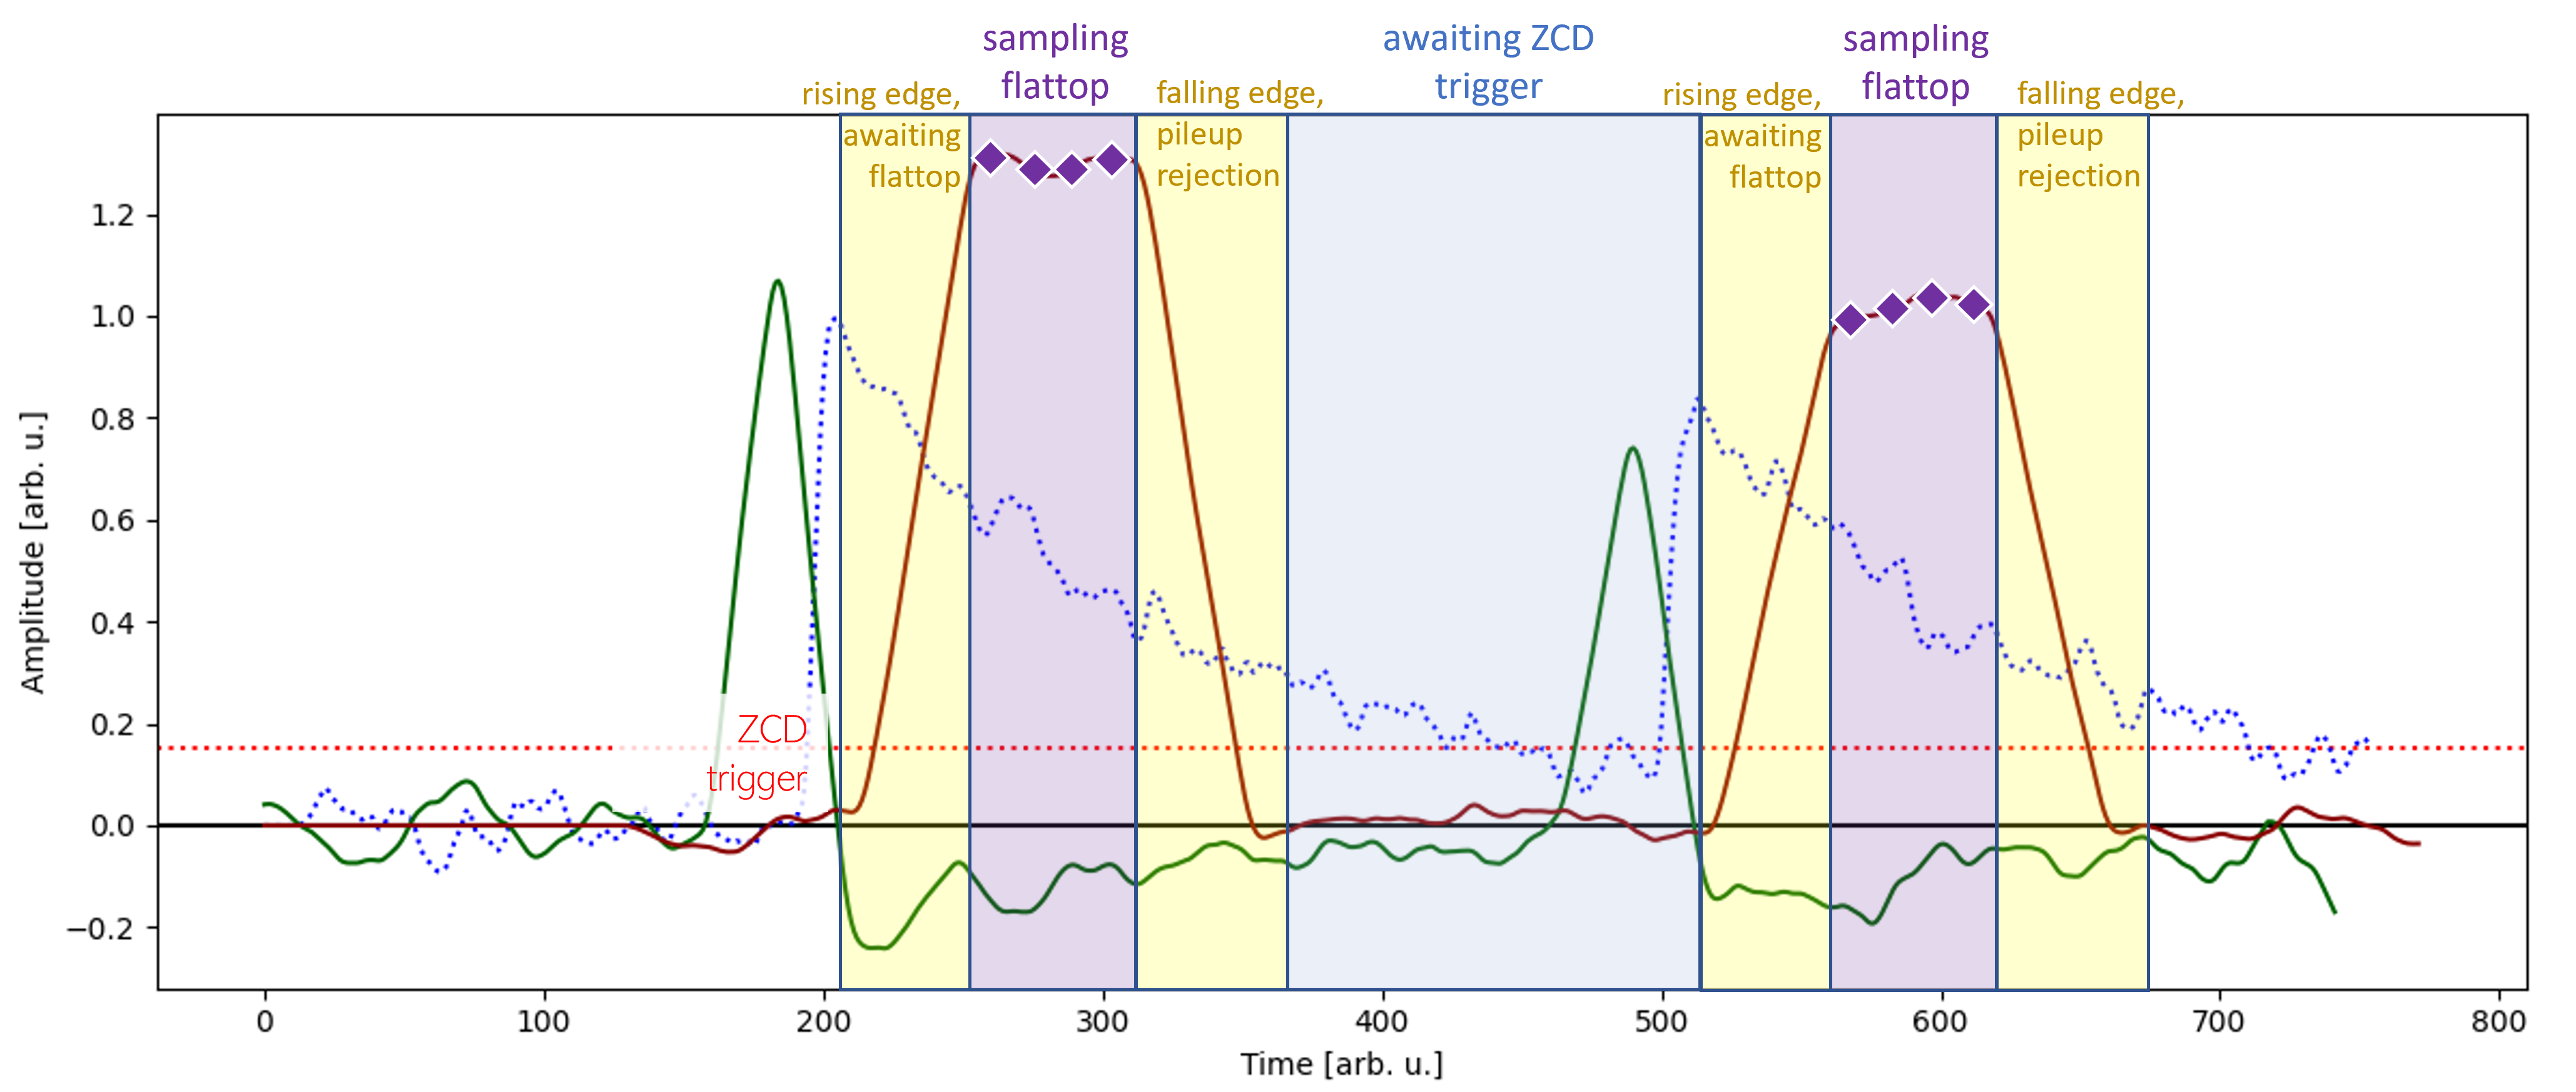
\includegraphics[width=\linewidth]{media/pha_algorithm.png}
  \caption{Trapezoid filter being used for pulse height analysis}
  \label{fig:pha_algorithm} 
\end{figure}


Instead of the complicated MWD algorithm, a hardware-optimized 
design of the trapezoidal filter, described by Jordanov \cite{jordanov_trapezoidal}
is used. \autoref{fig:trapezoid_dsp} shows the filter being 
implemented with the use of DSP blocks. The design requires two 
accumulators, four addition blocks and one multiplier.
Single-clock constant multiplication can be achieved with designs
based on Look Up Tables (LUTs). If the operand M is a power of 2,
the operation can be replaced with a left bit shift.
\begin{figure}[H]
  \centering
  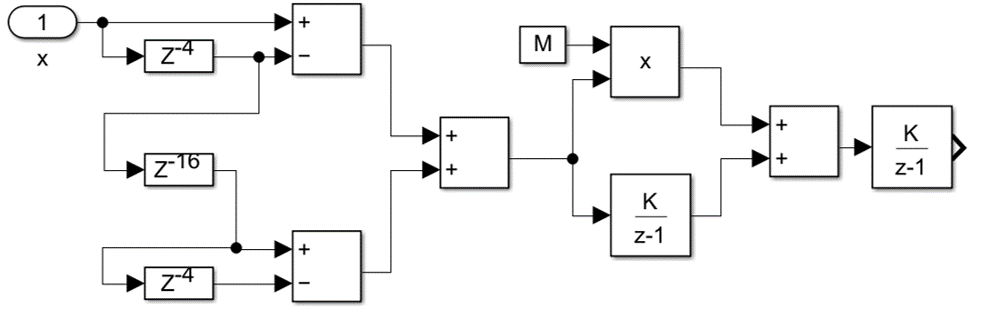
\includegraphics[width=\linewidth]{media/trapezoid_dsp.png}
  \caption{Trapezoid filter realized with the use of DSP blocks}
  \label{fig:trapezoid_dsp} 
\end{figure}

\subsubsection{Experimental results}

The custom PHA firmware was programmed onto ADQ14 and run in parallel
with an acquisition process. The firmware solution performed real-time
spectroscopy. At the same time the raw signal was transferred to the PC.
After an hour long acquisition finished, the raw signal was processed 
with a software algorithm and compared with the spectrum downloaded from the FPGA.


\autoref{fig:hardware_software_spectrum}
shows the results of the real-time firmware spectroscopy overlaid
with the offline processing method. The most important features
of the $^{137} Cs$ sample are preserved in the hardware spectrum,
suggesting a successful implementation of the described algorithm.
The proposed HXRM will be tested with other samples in the future.

\begin{figure}[H]
  \centering
  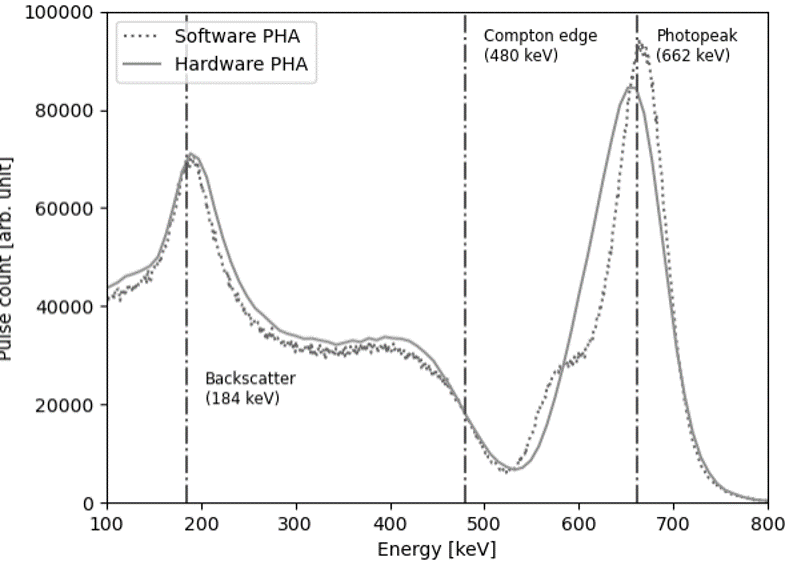
\includegraphics[width=\linewidth]{media/hardware_software_spectrum.png}
  \caption{Spectrum obtained with the developed HXRM module}
  \label{fig:hardware_software_spectrum} 
\end{figure}

\subsection{Spectrum storage and transfer}

The HXRM specification requires it to operate in continuous windowed mode.
Spectra are collected in 10 ms windows. As soon as one window finishes,
the device must start building a second spectrum, while simultaneously 
transferring the first one to the PC. No dead-time should occur 
when starting a new sampling window.


This requirement poses a problem when it comes to the spectrum storage.
With 14-bit samples the maximum theoretical resolution of the spectrum
that can be obtained is also going to be 14 bits. A spectrum is essentially 
an array of pulse counts in each bin range. With 32 bits chosen 
for the count resolution a total of $2^{14}$ 32-bit words is required to 
store a single spectrum.
This requires the use of Block Random Access Memory (BRAM)
as no other FPGA memory structure can realize
individually addressable increments on this scale within the timing constraints.


To prevent dead-time two BRAMs are used in an alternating mode.
While one of the BRAMs is used to build the spectrum, the other one
transfers its data to the PC and then resets its counts to back to zero.
Once a window finishes the roles are reversed.
\autoref{fig:bram_spectrum} shows the schematic view of this idea. 
For long spectrum acquisition and debugging purposes an additional third BRAM is used. 
This memory gets reset only on explicit user request.

\begin{figure}[H]
  \centering
  
\includegraphics[width=\linewidth]{media/bram_spectrum.png}
  \caption{Spectrum storage with three BRAMs}
  \label{fig:bram_spectrum} 
\end{figure}

The transfer and reset process requires the entire BRAM to be travelled twice. 
The ADQ14 can transfer 4 ADC samples or 64-bits of data
on each FPGA clock cycle for each channel to the internal FIFO RAM.
With 32-bit spectrum counts two bin counts can be transferred
on each clock cycle. To achieve that
both port interfaces have to be used to read two consecutive bins.
This behaviour requires the BRAM to be travelled once again after transferring
to reset all the count values to zero. This time both port interfaces
write zeros to two consecutive addresses. With a 4 ns clock period
the BRAM needs 33$\mu s$ to transfer its contents and another 33$\mu s$ to reset itself.

{\Huge [OBRAZEK]}
